\documentclass[10pt,twocolumn,letterpaper]{article}
\usepackage{wacv}
\usepackage{times}
\usepackage{epsfig}
\usepackage{graphicx}
\usepackage{amsmath}
\usepackage{amssymb}
\usepackage{subfig}
\usepackage{graphicx}
\usepackage{amsmath}
\usepackage{amssymb}
\usepackage{mathtools} % mathtools builds on and exten0))ds amsmath package
\usepackage{algpseudocode}	% http://ctan.org/pkg/algorithmicx% Include other packages here, before hyperref.
\usepackage{comment, url}
\usepackage{bm}
\usepackage[ruled, vlined, linesnumbered]{algorithm2e}
\newcommand{\forceindent}{\leavevmode{\parindent=1em\indent}}
\usepackage[hidelinks]{hyperref}

% Include other packages here, before hyperref.

% If you comment hyperref and then uncomment it, you should delete
% egpaper.aux before re-running latex.  (Or just hit 'q' on the first latex
% run, let it finish, and you should be clear).
%\usepackage[pagebackref=true,breaklinks=true,letterpaper=true,colorlinks,bookmarks=false]{hyperref}

\wacvfinalcopy % *** Uncomment this line for the final submission

\def\wacvPaperID{****} % *** Enter the wacv Paper ID here
\def\httilde{\mbox{\tt\raisebox{-.5ex}{\symbol{126}}}}

% Pages are numbered in submission mode, and unnumbered in camera-ready
\ifwacvfinal\pagestyle{empty}\fi
\setcounter{page}{1}
\begin{document}

%%%%%%%%% TITLE
\title{{\it E}nKCF: Ensemble of Kernelized Correlation Filters for
  High-Speed Object Tracking}

% Authors at the same institution
%\author{First Author \hspace{2cm} Second Author \\
%Institution1\\
%{\tt\small firstauthor@i1.org}
%}
% Authors at different institutions
\author{Burak Uzkent \\
Chester F. Carlson Center for Imaging Science\\
Rochester Institute of Technology\\
{\tt\small bxu2522@rit.edu}
\and
YoungWoo Seo \\
Independent Robotics Research (IR2)\\
{\tt\small youngwoo.blank.seo@gmail.com}
}

\maketitle
\ifwacvfinal\thispagestyle{empty}\fi

%%%%%%%%% ABSTRACT
\begin{abstract}
Computer vision technologies are very attractive for practical
applications running on embedded systems. For such applications, it is
desirable for the deployed algorithms to run in high-speed and require
no offline training. To develop a single-target tracking algorithm
with these properties, we propose an ensemble of the kernelized
correlation filters (KCF), we call it {\it E}nKCF. A committee of KCFs
is designed to specifically address the variations in scale and
translation of moving objects. To guarantee a high-speed run-time
performance, we deploy each of KCFs in turn, instead of applying
multiple KCFs to each frame altogether. To reduce any potential drifts
between individual KCFs' transition, we developed a particle
filter. Experimental results showed that 1) the performance of ours
is, on average, 70.10\% for precision at 20 pixels, 53.00\% for
success rate for the OTB100 data, and 54.50\% and 40.2\% for the
UAV123 data, and 2) our method is, on average, better than other
high-speed trackers over 5\% on precision on 20 pixels and 10-20\% on
AUC. In addition, our implementation ran at 340 fps for the OTB100 and
at 416 fps for the UAV123 dataset that is faster than DCF (333 fps)
for the OTB100 and KCF (296 fps) for the UAV123. To increase
flexibility of the proposed {\it E}nKCF running on various platforms,
we also explored different levels of deep convolutional features.
\end{abstract}

%%%%%%%%% BODY TEXT
\section{Introduction}
\label{introduction}
A recent advancement of air/ground/water unmanned vehicle technologies
has increased interests on deploying intelligent algorithms to
existing mobile platforms. Among those technologies, computer vision
algorithms are getting more attentions primarily because payloads of
those mobile platforms are limited to carry any other sensors than a
monocular camera. Instead of just manually being flew for video
recording, an unmanned air vehicle (UAV) equipped with an object or
feature following function would make it more useful for the
application of monitoring/surveillance/surveying on private
properties/wild-life/crop, video recording on various events, many
others. To this end, in this paper, we propose a single-target
tracking algorithm that does not require offline training and can run
at high-speed. Specifically, we would like to have our algorithm 1)
learn the appearance model of a target on the fly and 2) run on a
typical desktop as fast as $300$-$450$ fps.

\begin{figure*}[!h]
\centering
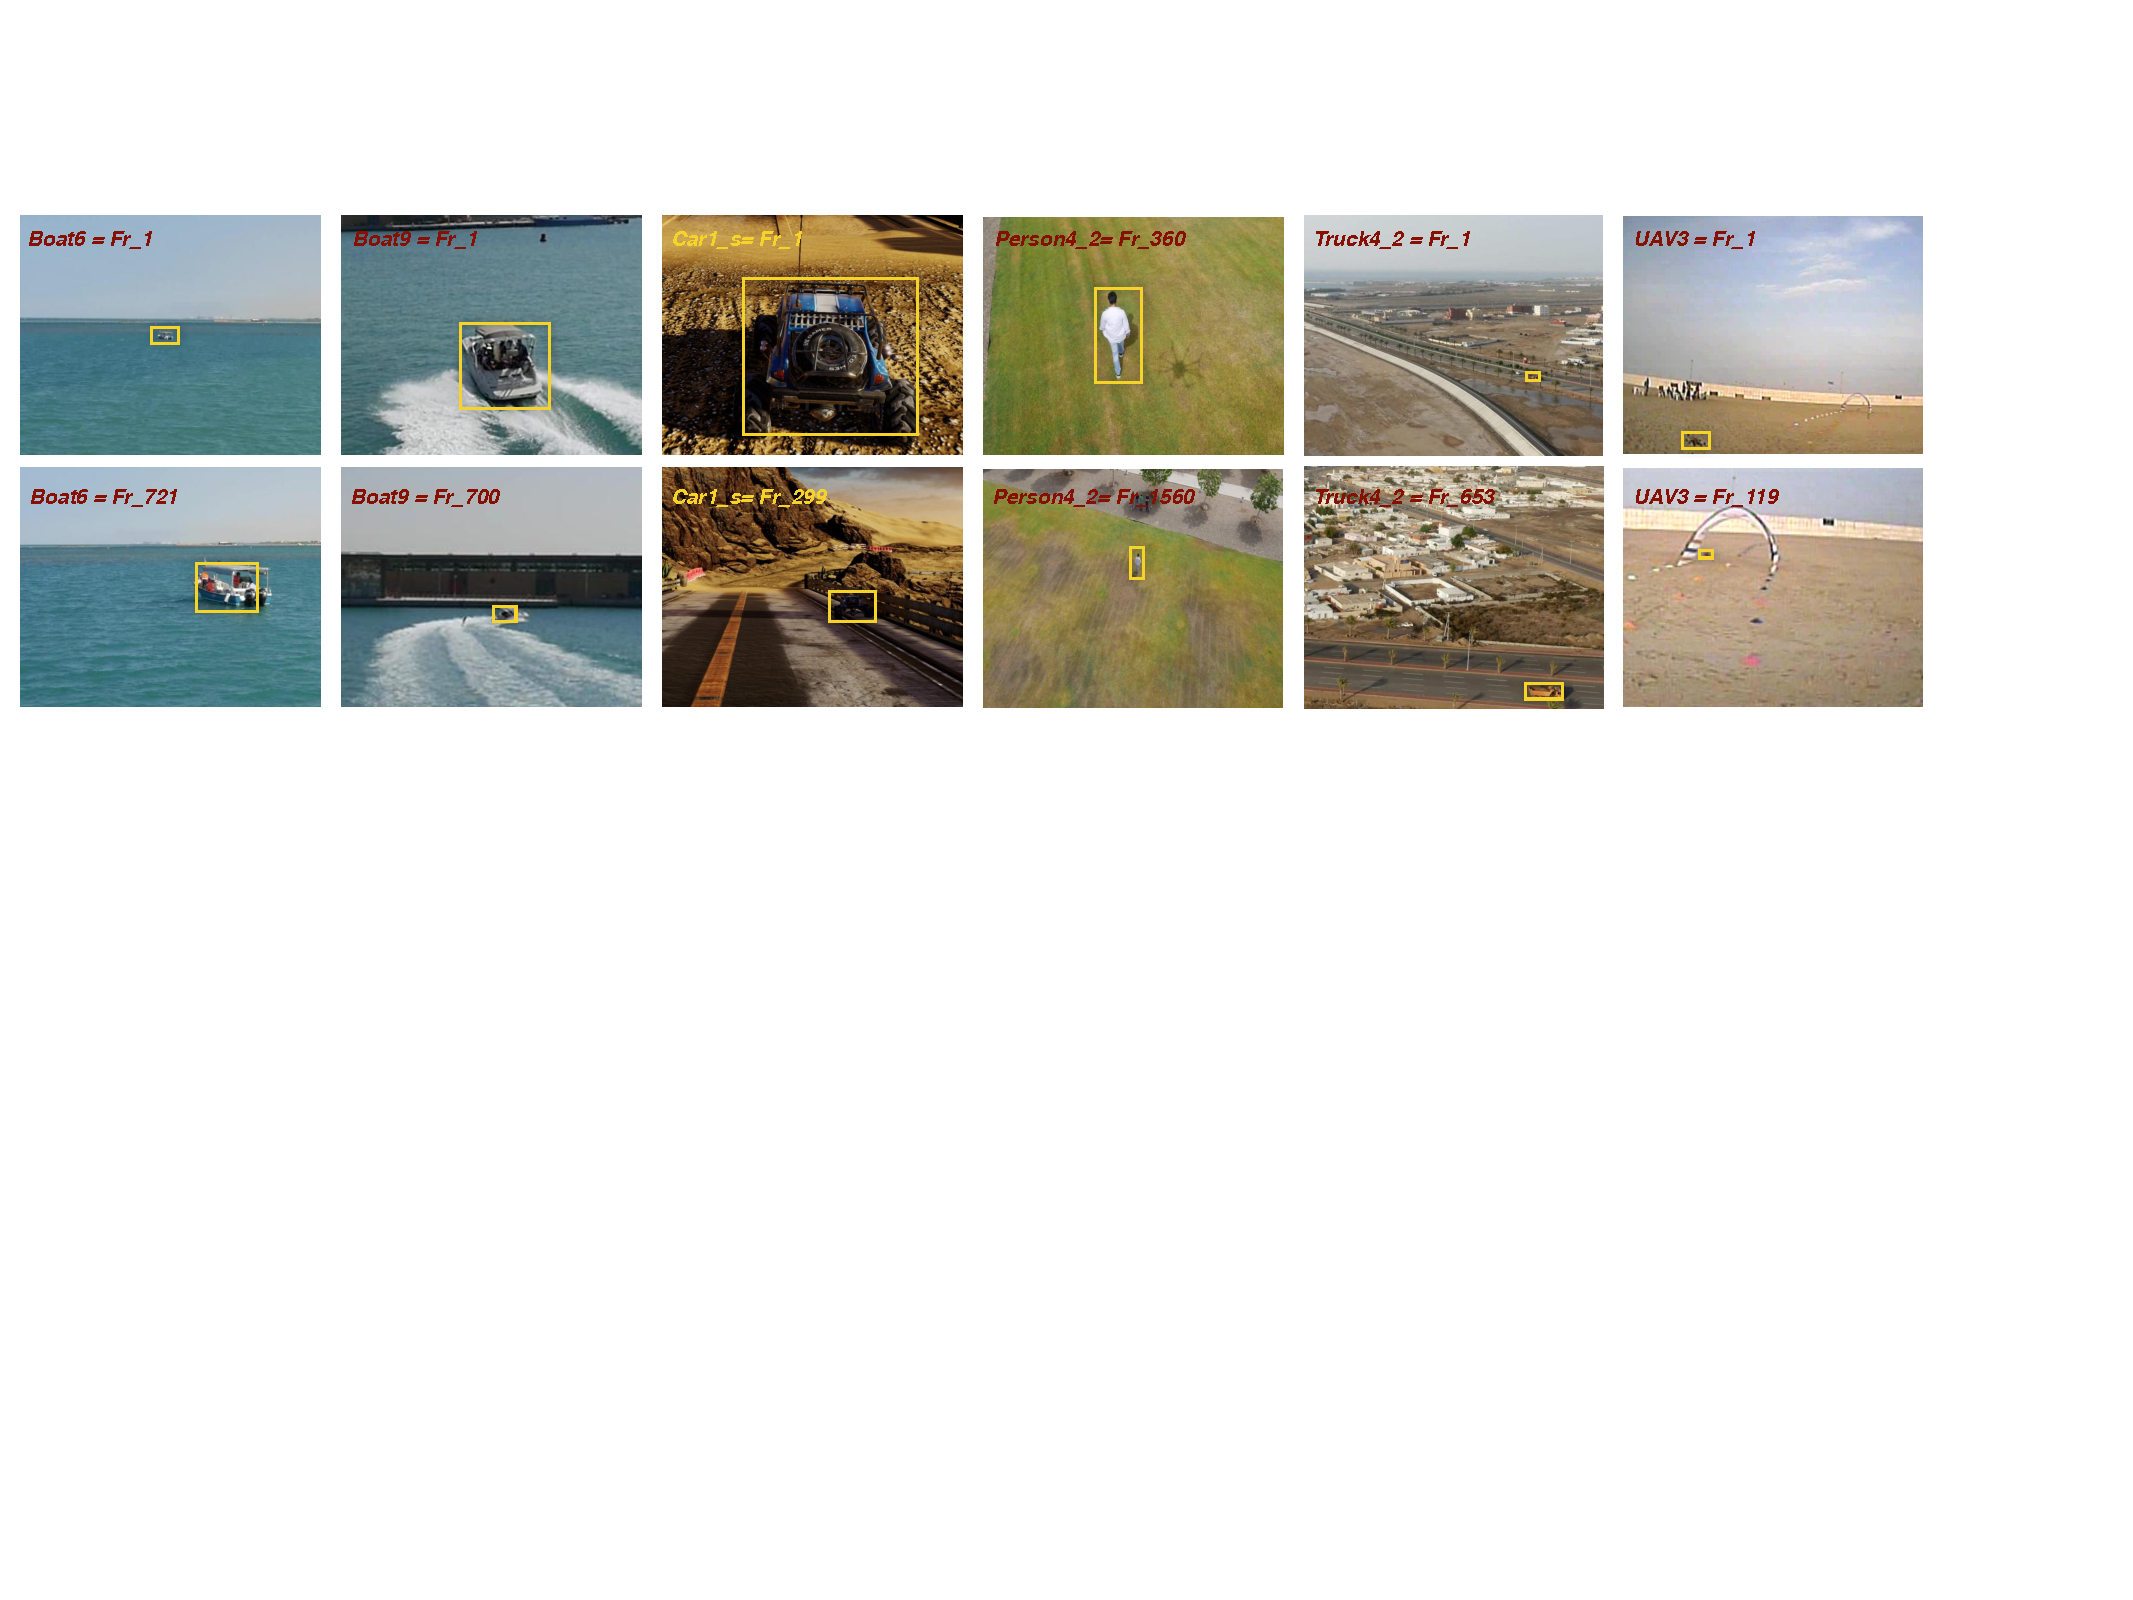
\includegraphics[width=\textwidth]{./figures/ResultsIntroduction.pdf}
\caption{Examples of some tracking results (yellow rectangles) by the
  proposed method on the ``UAV123'' dataset. The ``UAV123'' dataset is
  challenging for object tracking as the scale and translation of a
  target can be drastically changed in a few consecutive frames.}
\label{ResultsIntroduction}
\end{figure*}

\begin{figure*}[!h]
\centering
\begin{tabular}{cc}
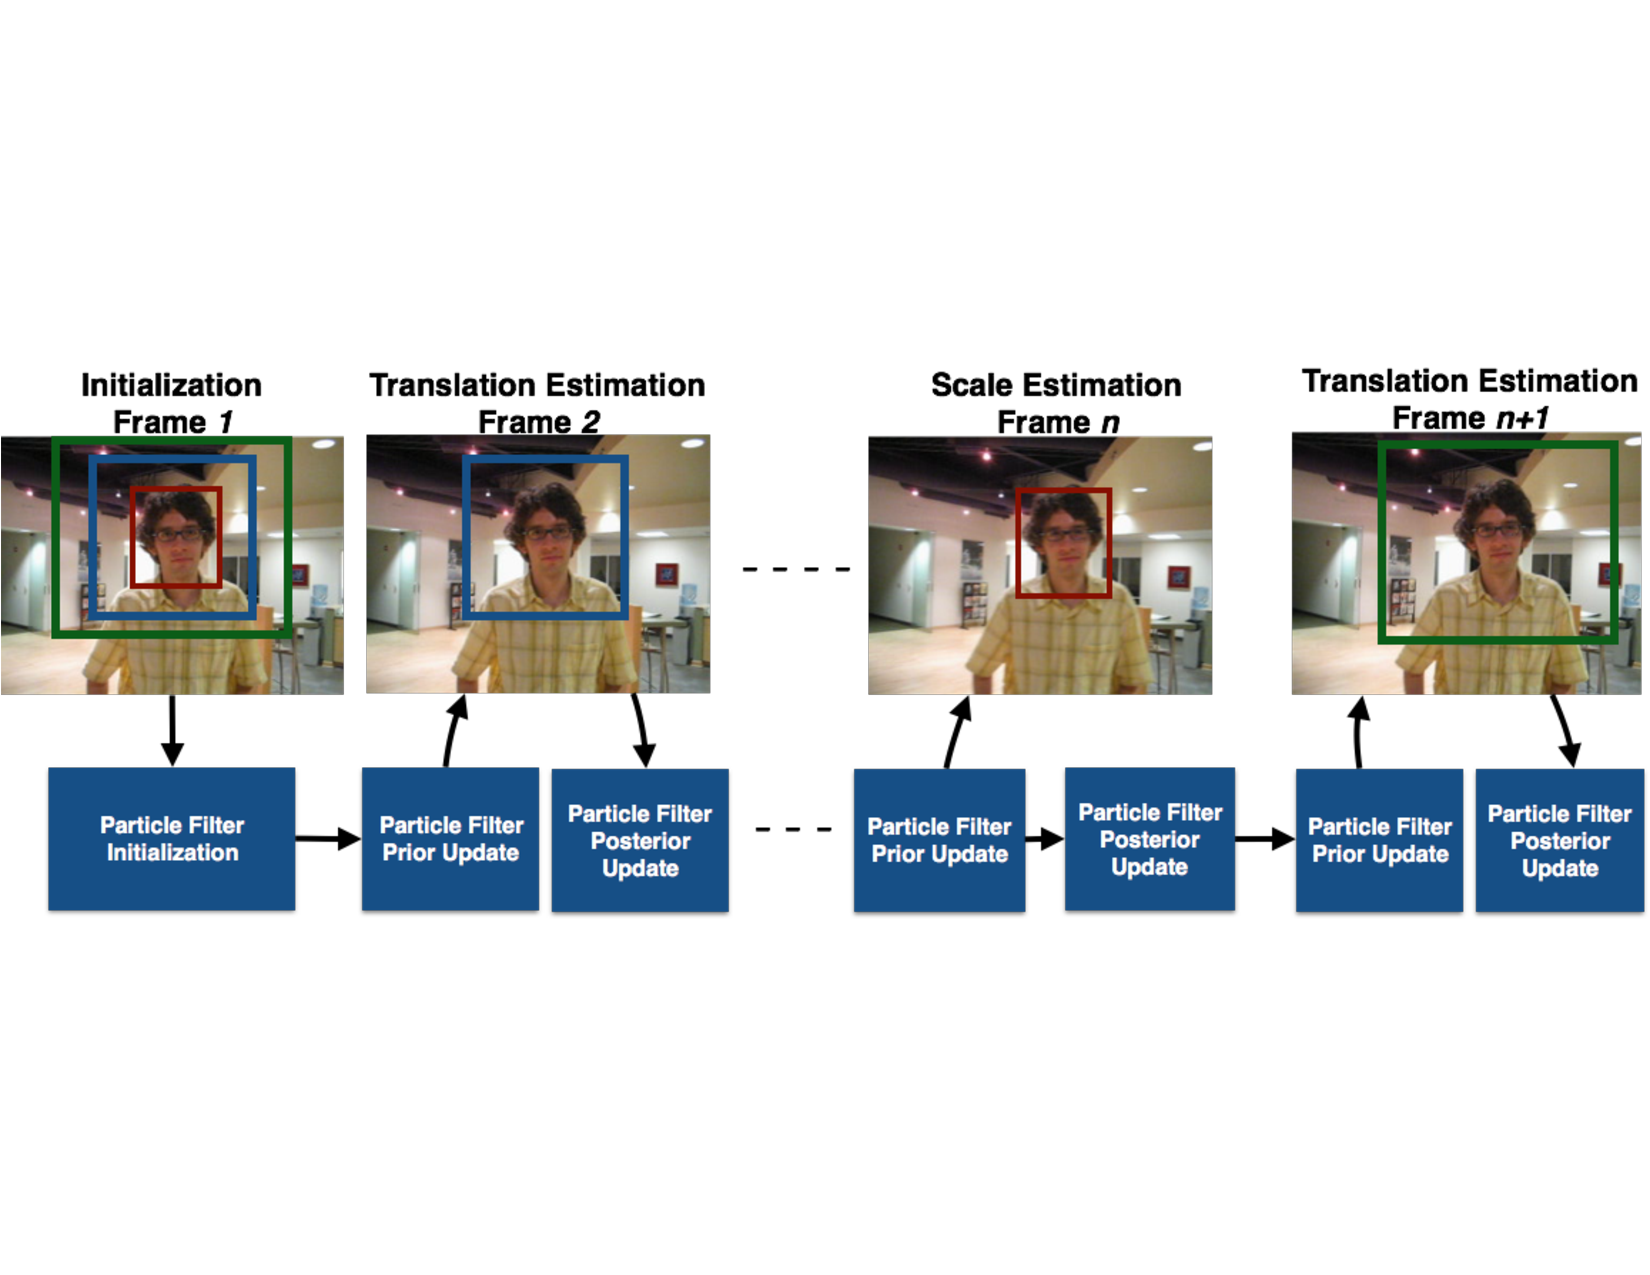
\includegraphics[width=14.00cm]{./figures/Workflow_MKCF+PF.pdf}\\
\end{tabular}
\caption{The workflow of the {\it E}nKCF. The first frame is used to
  initialize the tracking algorithm and a particle filter. For the
  next six frames, each of three KCF is deployed in turn to estimate
  the translation and scale change of a target. Afterward, the order
  of deploying three KCFs is repeating.}
\label{Workflows}
\end{figure*}

One of the dominant frameworks for online object tracking is the
correlation filter that essentially solves a single-target tracking
problem as a regression problem in the frequency domain. This method
assumes that a target location is given at the beginning like any
other online tracking algorithms \cite{smeulders2014survey}. Given
this positive example for the regression problem, a set of negative
examples is collected around the initial target bounding box and
represented as a form of the circulant matrix
\cite{henriques2015high}. One can optimally solve this regression
problem using a ridge regression in a closed form. However, this
solution has to deal with expensive matrix operations
$\mathcal{O}(n^{3})$. The correlation filter offers a less complex
solution, $\mathcal{O}(n\log n)$ by element-wise multiplication in a
frequency domain \cite{bolme2010visual,henriques2015high}. Thank to
this reformulation, an object tracking pipeline based on the
correlation filter can run very efficiently and be even easily
implemented. In fact, an extension of a linear correlation filter, the
kernelized correlation filter with multi-channel features
\cite{henriques2015high} showed impressive object tracking results and
outperformed other state-of-the-art, online tracking algorithms in
terms of run-time and tracking accuracy. However, a vanilla form of
such an online tracker is prone to drift, and fails to track a target
over a long period of time \cite{henriques2015high}. This is primarily
due to the dilemma of stability-plasticity in updating appearance
model, where the appearance model will be overfitted to only the
images used to train, unless a compromise on the frequency of updating
the model is carefully implemented \cite{santner2010prost}. For
example, one may handle a target's scale variation by just
concatenating multiple correlation filters including KCF and running
them on each frame. Alternatively one could think of scanning the
region of interest (ROI) with a list of templates in predefined scale
ratios to find the target in appropriate scale
\cite{bibi2015multi,henriques2015high,li2014scale,ma2015long,tang2015multi}. However,
these approaches would drastically reduce run-time performance because
multiple KCFs run on each frame.

Another way of handling the scale change for the correlation filter
based approach is to estimate a correct scale at a location where a
target highly likely appears \cite{zhang2014fast} -- estimate a
target's translation first and then estimate correct scale. For
example, Zhang and his colleagues used the MOSSE tracker
\cite{bolme2010visual} to estimate the target's translation. And then
their method updated the scale of the target by further analyzing
image sub-regions in high confidence. Their method is based on an
assumption that the scale of a target would not change drastically
over two consecutive frames. Similarly, Ma and his colleagues used two
KCFs to learn the translation and scale of a target separately
\cite{ma2015long}. In particular, a KCF is used to learn the
translation of the target and its background. Given this, another KCF
is used to learn the target area to estimate the new scale of the
target. However, because of running more than a KCF on each frame,
this method degrades its run-time performance (i.e., $\leq 50
fps$). Our method is motivated by this idea -- the idea of deploying
multiple KCFs to address the issues of single target tracking the
drastic variations in scale and translation, but in a more efficient
way. To maximize run-time performance and accuracy, instead of running
them all together on every frame, we deploy three KCFs in turn:
\textit{target}+\textit{small background} translation filter
($R_{t}^{S}$), \textit{target-only} scale filter ($R_{s}$) and
\textit{target}+\textit{large background} translation filter
($R_{t}^{L}$). By doing so, our method aims at effectively addressing
scale change and estimating target's motion while maintaining run-time
performance at high-speed. Figure \ref{Workflows} illustrates the
workflow of the {\it E}nKCF.

The contribution of this paper is a novel, single-target tracking
algorithm running at a very high-speed ($\geq300$ fps). In particular,
to effectively address the changes in scale and translation of a
target, we extended the KCF and deployed each of three KCFs in
turn. Because of such a deployment strategy, the run-time performance
of the proposed algorithm maintains high without sacrificing the
accuracy of tracking. To reduce any potential drifts while switching
KCFs, we developed a particle filter. Additionally, to increase the
flexibility of the proposed algorithm's usage, we explore deep
convolutional features with varying levels of abstraction.

%---------------------------------------------------------------------- 
\section{{\it E}nKCF: Ensemble of Kernelized Correlation Filters}
%---------------------------------------------------------------------- 
We propose a novel way of utilizing an ensemble of the KCFs
\cite{henriques2015high} to effectively handle scale variations and
dynamic maneuvers of a target. To improve the run-time performance and
maintain the small-footprint of the original KCF (e.g., $\ge$ 300), we
deploy three KCFs in turn, instead of applying them altogether on the
same image frame. Each of these KCFs is designed to address the
challenges of single-target tracking -- variance in scale and
translation.

\begin{algorithm*}[h]
\small
\DontPrintSemicolon
\KwIn{ Initial bounding box $(x_{0},y_{0},s_{0})$, frame counter $fc$, complete cycle of scale filter $n = 5$,}
\KwOut{	\uIf{$fc\:\%\:n=0$ (\textbf{Condition 1})}
			{
				Estimated Target State $(x_{t},y_{t},s_{t})$,
				Scale filter (\textit{target-only}) model $R_{s}$
			}
			 \ElseIf{$fc\:\%\:n>0\:\:and\:\:fc\:\%\:n\leq n/2$ (\textbf{Condition 2})}
			 {
				Estimated Target State $(x_{t},y_{t},s_{t} = s_{t-1})$,
			  	Large Area Translation Filter model $R_{t}^{L}$
			}			 
			 \Else (\textit{\textbf{Condition 3}})
			{			 
				 Estimated Target State $(x_{t},y_{t},s_{t} = s_{t-1})$,
				Small Area Translation Filter model $R_{t}^{S}$			
			}	
		}
\SetKwBlock{Begin}{function}{end function}
\Begin($\text{track($x_{t-1},y_{t-1},s_{t-1}$) }$)
{
 	// \textit{Translation Estimation - Particle Filter} \\
	Transit Particle Filter to the frame $t$ and compute the mean of prior pdf $(x_{t},y_{t},s_{t-1})$ \\
     // \textit{Translation Estimation - Correlation Filter} \\
	Crop the ROI for the $R_{t}^{L}$ (Condition 2), or $R_{t}^{S}$ (Condition 3) given $(x_{t},y_{t})$ and estimate new position as $(x_{t},y_{t})$ = $\mathbf{\textit{max}(y_{R_{t}})}$\\
	// \textit{Scale Estimation - Correlation Filter}\\
	Scale pool for $R_{s}$ : $\mathbf{S} = \lbrace1.05,1.0,1/1.05\rbrace$,\\
	Crop the ROI for the $R_{s}^{i}$ (Condition 1) and estimate scale factor, $\mathbf{\alpha}$ = $\underset{i\in S}{\textit{argmax}}(PSR(\boldsymbol{y_{R_{s}^{i}}}))$, and new scale $s_{t} = \alpha * s_{t-1}$,\\ 
	// \textit{Update Translation - Particle Filter}\\
	Do Importance Re-sampling (if necessary) and compute the 
	mean of posterior pdf $(x_{t},y_{t})$\\
	// \textit{Model Update}\\
	Update $R_{t}^{S}$ (Condition 3),\\
	Update $R_{t}^{L}$ (Condition 2),\\
	\uIf{$PSR(\boldsymbol{y_{R_{s}}}) \geq T_{R_{s}}$}{
		Update $R_{s}$ (Condition 1)}
  \label{endfor}
  \Return{($x_{t},y_{t},s_{t}$)}
}
\caption{{\it E}nKCF Tracking Algorithm}\label{alg:MKCF}
\end{algorithm*}

The proposed algorithm, {\it E}nKCF, learns three KCFs in turn: The
first filter, $R_{t}^{S}$, focuses on learning the target area and its
background for addressing a marginal translation of a target, the
second filter, $R_{s}$, focuses entirely on learning the target's
scale, and the last filter, $R_{t}^{L}$, focuses on the target area
and its background bigger than that of the first filter,
$R_{t}^{S}$. By designing {\it E}nKCF as a composite of three KCFs, a
transition filter with larger padding size, $R_{t}^{L}$, will enable
{\it E}nKCF to recover from potential drifts after a scale filter,
$R_{s}$, is applied to the input images. Another translation filter
with smaller padding size, $R_{t}^{S}$, will help {\it E}nKCF to
better localize the position of the target after the large ROI
translation filter is applied. Our approach is similar to that of
\cite{ma2015long} which sequentially applied more than one KCF to
every frame, but different in that we operate multiple KCFs in an
alternating manner. It is intuitive to alternate multiple KCFs with
different goals over a small temporal window of the input image
sequences, because the appearance of a target does not change
drastically over consecutive images. In other words, for most cases,
learning a correlation filter over consecutive frames would not be
substantially different from the one updated with smaller
frequency. Figure \ref{fig:Filters_Comparison} shows examples
supporting this observation.

\begin{figure*}[!h]
\centering
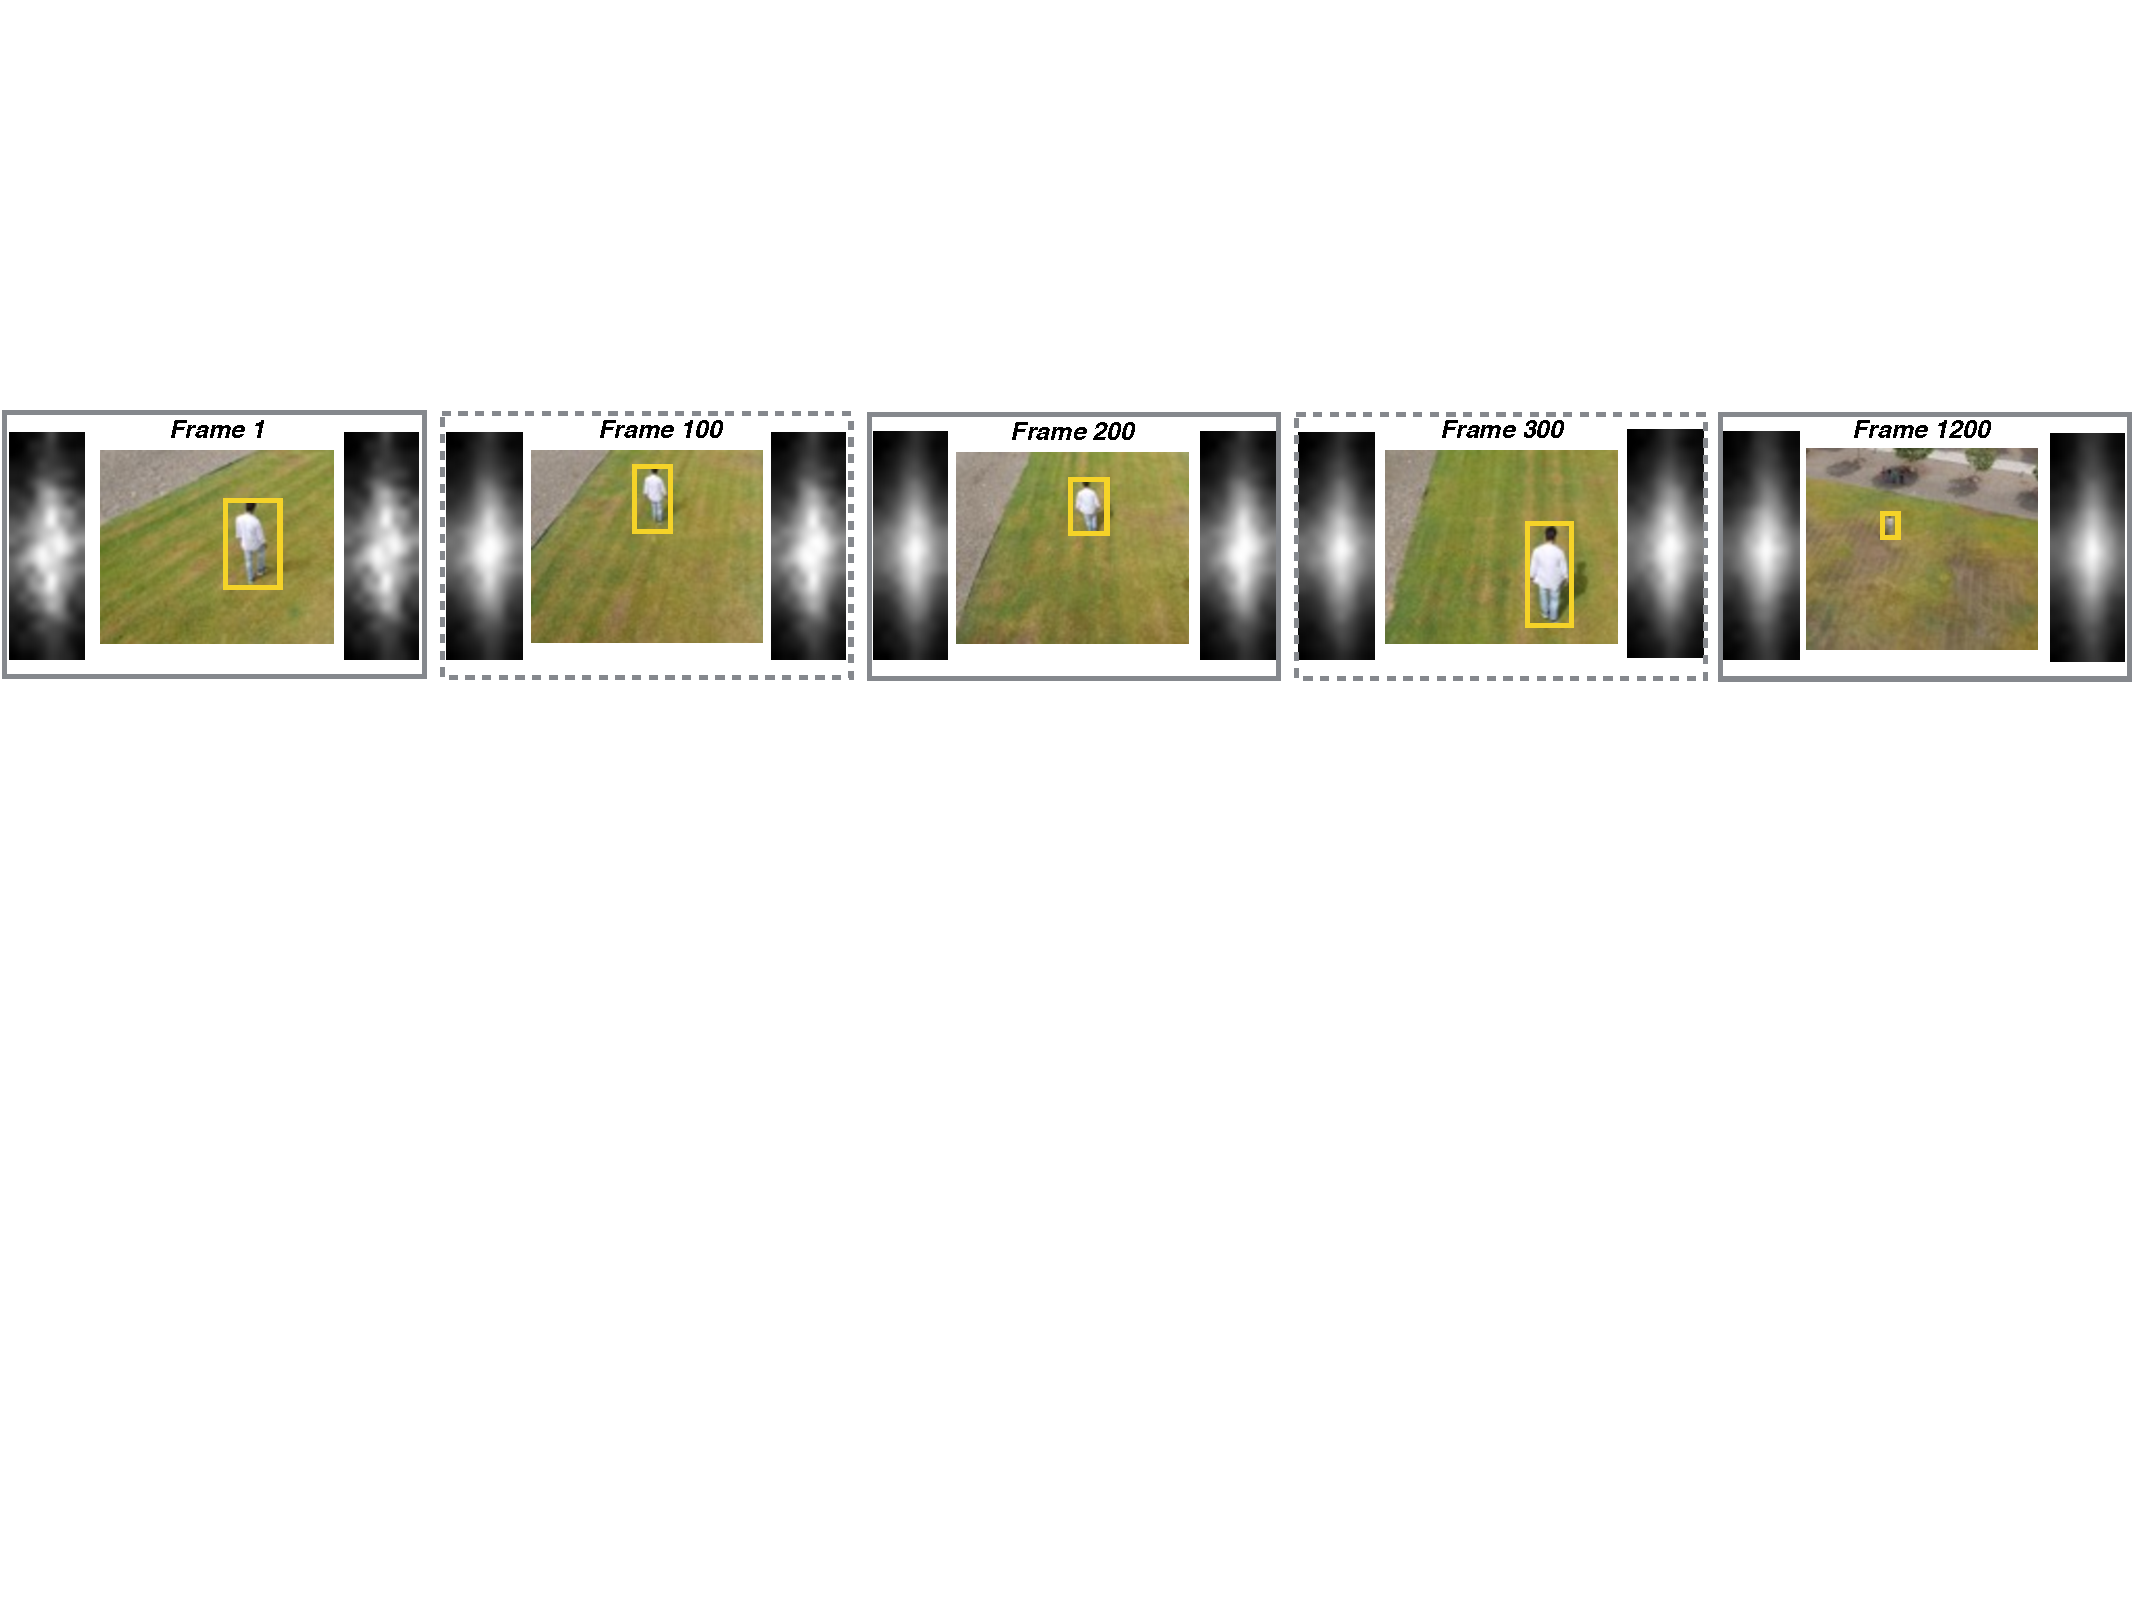
\includegraphics[width=1\textwidth]{./figures/LearnedFiltersComparison2.pdf}
\caption{These examples show that there is a marginal difference
  between the scale filters learned at every frame and the one learned
  at every 5 frames. In each figure, the leftmost, sub-figures show
  the scale filters trained at every frame and those at the rightmost
  show the scale filters trained at every 5 frames.}
\label{fig:Filters_Comparison}
\end{figure*}

The algorithm \ref{alg:MKCF} shows the pseudo-code of {\it E}nKCF.
The order of running these three KCFs is important because each of
these filters aims at addressing different challenges of single-target
tracking. A translation filter, $R_{t}^{L}$, is applied to the $i$th
and $i$+$1$th image frames, another translation filter, $R_{t}^{S}$,
is applied to the $i$+$2$th and $i$+$3$th image frames, and then the
scale filter, $R_{s}$, is applied to the $i$+$4$th image. This order
repeats until the last image of an input video is presented. Note that
the translation filter, $R_{t}^{L}$, is intended to run right after
the scale filter, $R_s$, runs which is applied at every other $i$+$4$
frames. We run these filters in this way because we want to minimize
any drifts that are likely to happen running only $R_{s}$. In
addition, the filter, $R_{t}^{S}$, is applied to every other two
frames before $R_{s}$ and right after two consecutive frames running
$R_{t}^{L}$. By repeating this order of learning three KCFs, we can
integrate more discriminating shape features that cannot be learned
just by $R_{t}^{L}$. The filter, $R_{t}^{L}$, uses shape and color
information together to recover from any potential drifts -- drifts
could happen due to only scale filter operation in certain frames.

In summary, the scale filter, $R_{s}$, is designed to directly handle
the scale change of a target and provides the translation filters,
$R_{t}^{L}$ and $R_{t}^{S}$, with more accurate ROIs. On the other
hand, a translation filter, $R_{t}^{L}$, is devised to look into a
larger search area to estimate the target's translation and recover
from any potential drifts. Another translation filter, $R_{t}^{S}$, is
designed to address the drawback of $R_{t}^{L}$ that may learn noisy
shape features due to its relatively larger search area. In what
follows, we will brief the main idea behind the KCF.

\textbf{Kernelized Correlation Filter} The Kernelized Correlation
Filter is a well-known single target tracking algorithm. As its
workflow has been detailed in other papers
\cite{henriques2012exploiting,henriques2015high}, in this section we
briefly go over the parts of the KCF relevant to this study. Its
computational efficiency is derived from the correlation filter
framework representing training examples as a circulant matrix. The
fact that a circulant matrix can be diagonalized by Discrete Fourier
transform is the key to reduce the complexity of any tracking method
based on correlation filter. The off-diagonal elements become zero
whereas the diagonal elements represent the eigenvalues of the
circulant matrix. The eigenvalues are equal to the DFT transformation
of the base sample ($\boldsymbol{x}$) elements. The Kernelized
Correlation Filter, in particular, applies a kernel to
$\boldsymbol{x}$ to transform into a more discriminating domain. The
circulant matrix is then formed by applying cyclic shifts on the
kernelized $\boldsymbol{x}$. Such kernelization operation maintains
$\mathcal{O}$($nlog(n)$) complexity unlike other kernel algorithms
leading to $\mathcal{O}$($n^{2}$) or even higher complexities.

The KCF solves essentially the problem of a regression in the form of
the regularization (ridge regression):
\begin{equation}
E_h = \min_{\boldsymbol{h}}\frac{1}{2}||\boldsymbol{y}-\sum_{c=1}^{C}\boldsymbol{h_{c}}*\boldsymbol{x_{c}}||^{2} + \frac{\lambda}{2}\sum_{c=1}^{C}||\boldsymbol{h_{c}}||^{2}
\label{eq:Closedform_RidgeReg}
\end{equation}
where we seek for $\boldsymbol{h}$ that minimizes $E$ given the
desired continuous response, $\boldsymbol{y}$, and the training
template $\boldsymbol{x}$.  The parameter $c$ enables one to integrate
features in the form of multiple channels, such as HoG and color, in
this setup \cite{galoogahi2013multi,henriques2015high}. To simplify
the closed-form solution for Equation \ref{eq:Closedform_RidgeReg}, an
element-wise multiplication in frequency domain was proposed to learn
the frequency domain correspondence of $\boldsymbol{h}$,
$\boldsymbol{\hat{w}}$:
\begin{equation}
\boldsymbol{\hat{w}} = \boldsymbol{\hat{x}^{*}}*\boldsymbol{\hat{y}}(\boldsymbol{\hat{x}^{*}}*\boldsymbol{\hat{x}}+\lambda)^{-1}.
\label{eq:DiagonalizedPrimalSolution}
\end{equation}
Where $*$ is an element-wise multiplication. A non-linear version of
$\boldsymbol{\hat{w}}$ and $\boldsymbol{\hat{\alpha}}$ are proposed to
increase robustness to any geometric and photometric variations
\cite{henriques2015high}. In particular, the diagonalized non-linear
Fourier domain dual form solution is expressed as
\begin{equation}
\boldsymbol{\hat{\alpha}} = \boldsymbol{\hat{y}}(\boldsymbol{\hat{k}^{xx^{'}}}+\lambda)^{-1}
\label{eq:FourierDualDomainSolution}
\end{equation}
where $\lambda$ represents the regularization weight whereas $\boldsymbol{\hat{k}^{xx^{'}}}$ denotes
 the first row of the kernel matrix $\boldsymbol{K}$ known as \textit{gram matrix} and is expressed as
\begin{equation}
\boldsymbol{k^{xx^{'}}} = exp(-\dfrac{1}{\alpha^{2}}(||\boldsymbol{x}||^{2}+||\boldsymbol{x}^{'}||^{2}-2F^{-1}(\sum^{C}_{c}\boldsymbol{\hat{x}_{c}}^{*}\odot \boldsymbol{\hat{x}_{c}}^{'}))).
\label{eq:GaussianCorrelationSingleChannel}
\end{equation}
An earlier version based on this formulation used grayscale feature
($C=1$) to learn the solution vector $\boldsymbol{w}$ and integrating
multi-channel features such as HoG and Color showed improved accuracy
\cite{bibi2015multi,galoogahi2013multi,henriques2015high,ma2015long,tang2015multi}.
In the detection step, the learned correlation filter is correlated
with the first row of the gram matrix, $\boldsymbol{k^{xz^{'}}}$,
which contains the similarity values between the learned feature
template $\boldsymbol{x}$ and the new test template
$\boldsymbol{z}$. This can be formulated as
\begin{equation}
\boldsymbol{r(z)} = F^{-1}(\boldsymbol{\hat{k}^{xz^{'}}} \odot \boldsymbol{\hat{\alpha}})
\end{equation}
where $\boldsymbol{r}$ denotes the correlation response at all cyclic shifts of the
first row of the kernel matrix.

To integrate further temporal information into tracker, we update the
correlation filter and the appearance model as below:
\begin{align}
\boldsymbol{\hat{\alpha}_{t}} = (1-\beta) \boldsymbol{\hat{\alpha}_{t-1}} + \beta \boldsymbol{\hat{\alpha}_{t}} \\
\boldsymbol{\hat{x}_{t}} = (1-\beta) \boldsymbol{\hat{x}_{t-1}} + \beta \boldsymbol{\hat{x}_{t}}
\end{align}
%\end{comment}
where $\beta$ represents the learning rate tuned to a small value in practice.

In the following sections, we will detail two different types of
features used in {\it E}nKCF: hand-crafted features (fHoG +
color-naming) and deep convolutional features.

\textbf{{\it E}nKCF with Hand-Crafted Features} We, first, use two
conventional hand-crafted features, fHoG (shape)
\cite{felzenszwalb2010object} and color-naming (color)
\cite{li2014scale}. Figure \ref{fig:Filters} shows examples of these
features. This setup of the {\it E}nKCF is designed to develop an
online tracking algorithm running at high-speed ($\ge$ 300 fps) on a
typical desktop (and eventually running $\ge 30$ fps on a low-end
embedded system without GPUs).
\begin{figure}[!h]
\centering
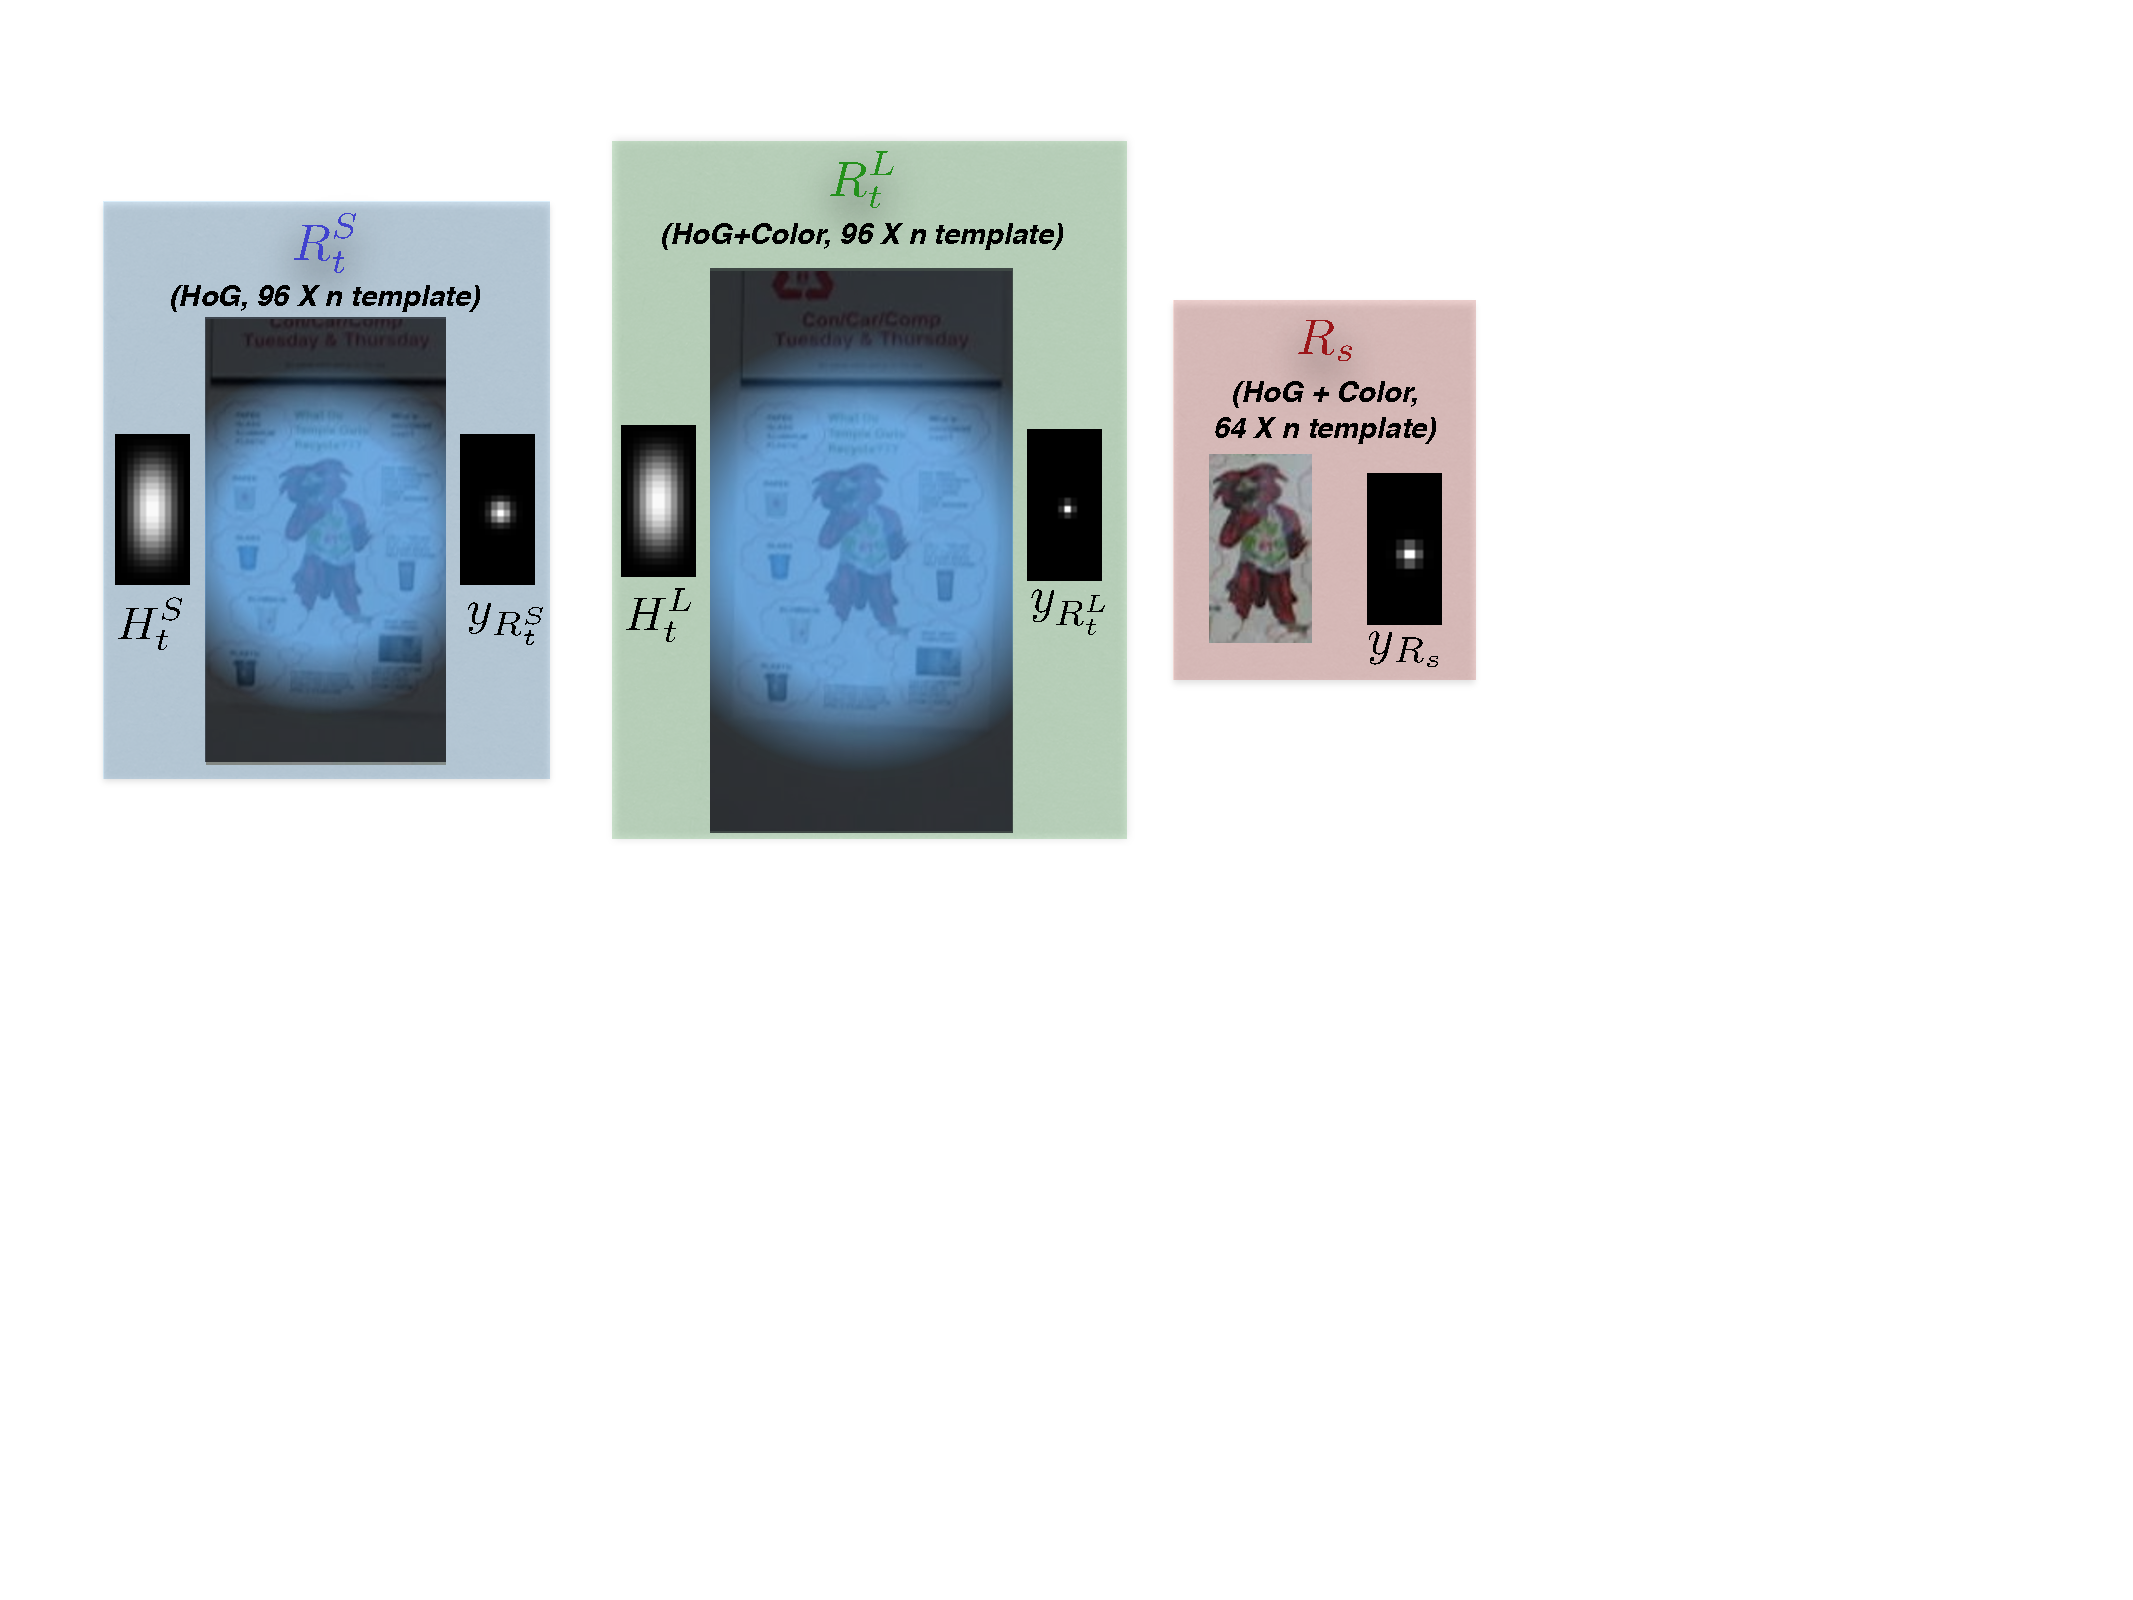
\includegraphics[width=0.47\textwidth]{./figures/Filters_Details.pdf}
   \\[-3ex]
\subfloat[Small area translation filter]{\hspace{.30\linewidth}}\label{fig:Rt_S}
\quad\subfloat[Large area translation filter]{\hspace{.37\linewidth}}\label{fig:Rt_L}
\quad\quad\subfloat[Scale filter]{\hspace{.12\linewidth}}\label{fig:Rs}
\caption{Examples of three filters with hand-crafted features. The
  responses by the large and small area translation filters, and scale
  filter represented by $y_{R_{t}^{L}}$, $y_{R_{t}^{S}}$ and
  $y_{R_{s}}$.}
\label{fig:Filters}
\end{figure}

We use both fHoG \cite{felzenszwalb2010object} and color-naming
\cite{van2009learning} for the large area translation filter,
$R_{t}^{L}$. This is because the fHoG tends to be noisier and less
discriminating, when it is applied to relatively larger area, and
adding color information makes the feature vector for the translation
filter more discriminating. Figure \ref{fig:Filters} (b) shows an
example of this translation filter. By contrast, the $R_{t}^{S}$ only
uses the fHoG features because it covers a relatively smaller area.
Figure \ref{fig:Filters} (a) shows an example of this translation
filter. Lastly, we use both fHoG and color-naming features again for
the scale filter, $R_{s}$. By assigning fHoG and color-naming
features, we ensure that the likelihood of inaccurate scale estimation
is decreased in comparison to the scale filter with only fHoG
features. This is more important in our case as the scale filter is
operated in every 5 frames. Also, the scale filter, explained earlier
in the algorithm \ref{alg:MKCF}, estimates the scale of a target by
correlating it with three candidate ROIs. This search may increase the
run-time complexity of the scale filter from $\mathcal{O}(n\log n)$ to
$\mathcal{O}(3(n\log n))$. To ensure practically feasible operations,
we use a smaller template size (i.e., 64$\times n$) for the scale
filter, $R_{s}$. The smaller template size does not degrade the
tracking performance because of 1) zero padding around the target
(smaller ROI) and 2) usage of color-naming features.

\textbf{{\it E}nKCF with Deep Convolutional Features} In addition to
hand-crafted features, we explore deep convolutional features to
extend the applicability of the {\it E}nKCF and boost tracking
performance.

There has been a large volume of studies on utilizing a pre-trained
CNN features for tracking-by-detection algorithms. For example,
\cite{danelljan2015convolutional} used the activation of the first and
second convolutional layer of the VGGNet \cite{simonyan2014very}.
They reported that the first convolutional layer features lead to
slightly better precision and success rates than the second layer due
to increased invariance for translation in this
layer. \cite{ma2015hierarchical} proposed a KCF tracker integrating
features with higher abstraction capacity. Their method, firstly used
the third convolutional layer features to estimate the response
map. In the next step, the KCF, concentrating on the second
convolutional layer features, ran to update transition. The third KCF
then worked on the transition given by the previous KCF, and learned
the first convolutional layer features to update the transition. This
coarse-to-fine translation estimation accommodates different levels of
abstractions of the object. However, their method runs multiple KCFs
in a sequential fashion, increasing the run-time complexity. For this
reason, we follow an approach similar to
\cite{danelljan2015convolutional}, in order to embed deep features in
     {\it E}nKCF. The {\it E}nKCF algorithm enables us to exploit
     different level of feature encodings with different KCFs. The
     translation filters, $R_{t}^{L}$ and $R_{t}^{S}$, consider at
     least twice bigger area than the scale filter, $R_{s}$. Given
     this, we can assign deeper feature encodings to $R_{s}$ as it
     learns less spatial information than $R_{t}^{L}$ and
     $R_{t}^{S}$. Thus we assign the activation of the fourth
     convolutional layer features ($26\times26\times128$) to $R_{s}$
     whereas $R_{t}^{L}$ and $R_{t}^{S}$ are assigned the activation
     of the second layer features ($109\times109\times64$). Figure
     \ref{fig:Filters_CNN} illustrates this feature
     assignment. Additionally, we assign the second convolutional
     layer features to $R_{s}$ as in $R_{t}^{L}$ and $R_{t}^{S}$ and
     compare this setting (\textit{conv222-VGG}) to
     \textit{conv224-VGG}, where the \textit{conv222} setting
     represents the assignment of the activation of $2^{th}$
     convolutional layer features of VGGNet to $R_{t}^{L}$,
     $R_{t}^{S}$ and $R_{s}$. We use the VGGNet since it provides
     higher spatial resolution at the first several layers than
     AlexNet \cite{krizhevsky2012imagenet}.

\begin{figure}[!h]
\centering
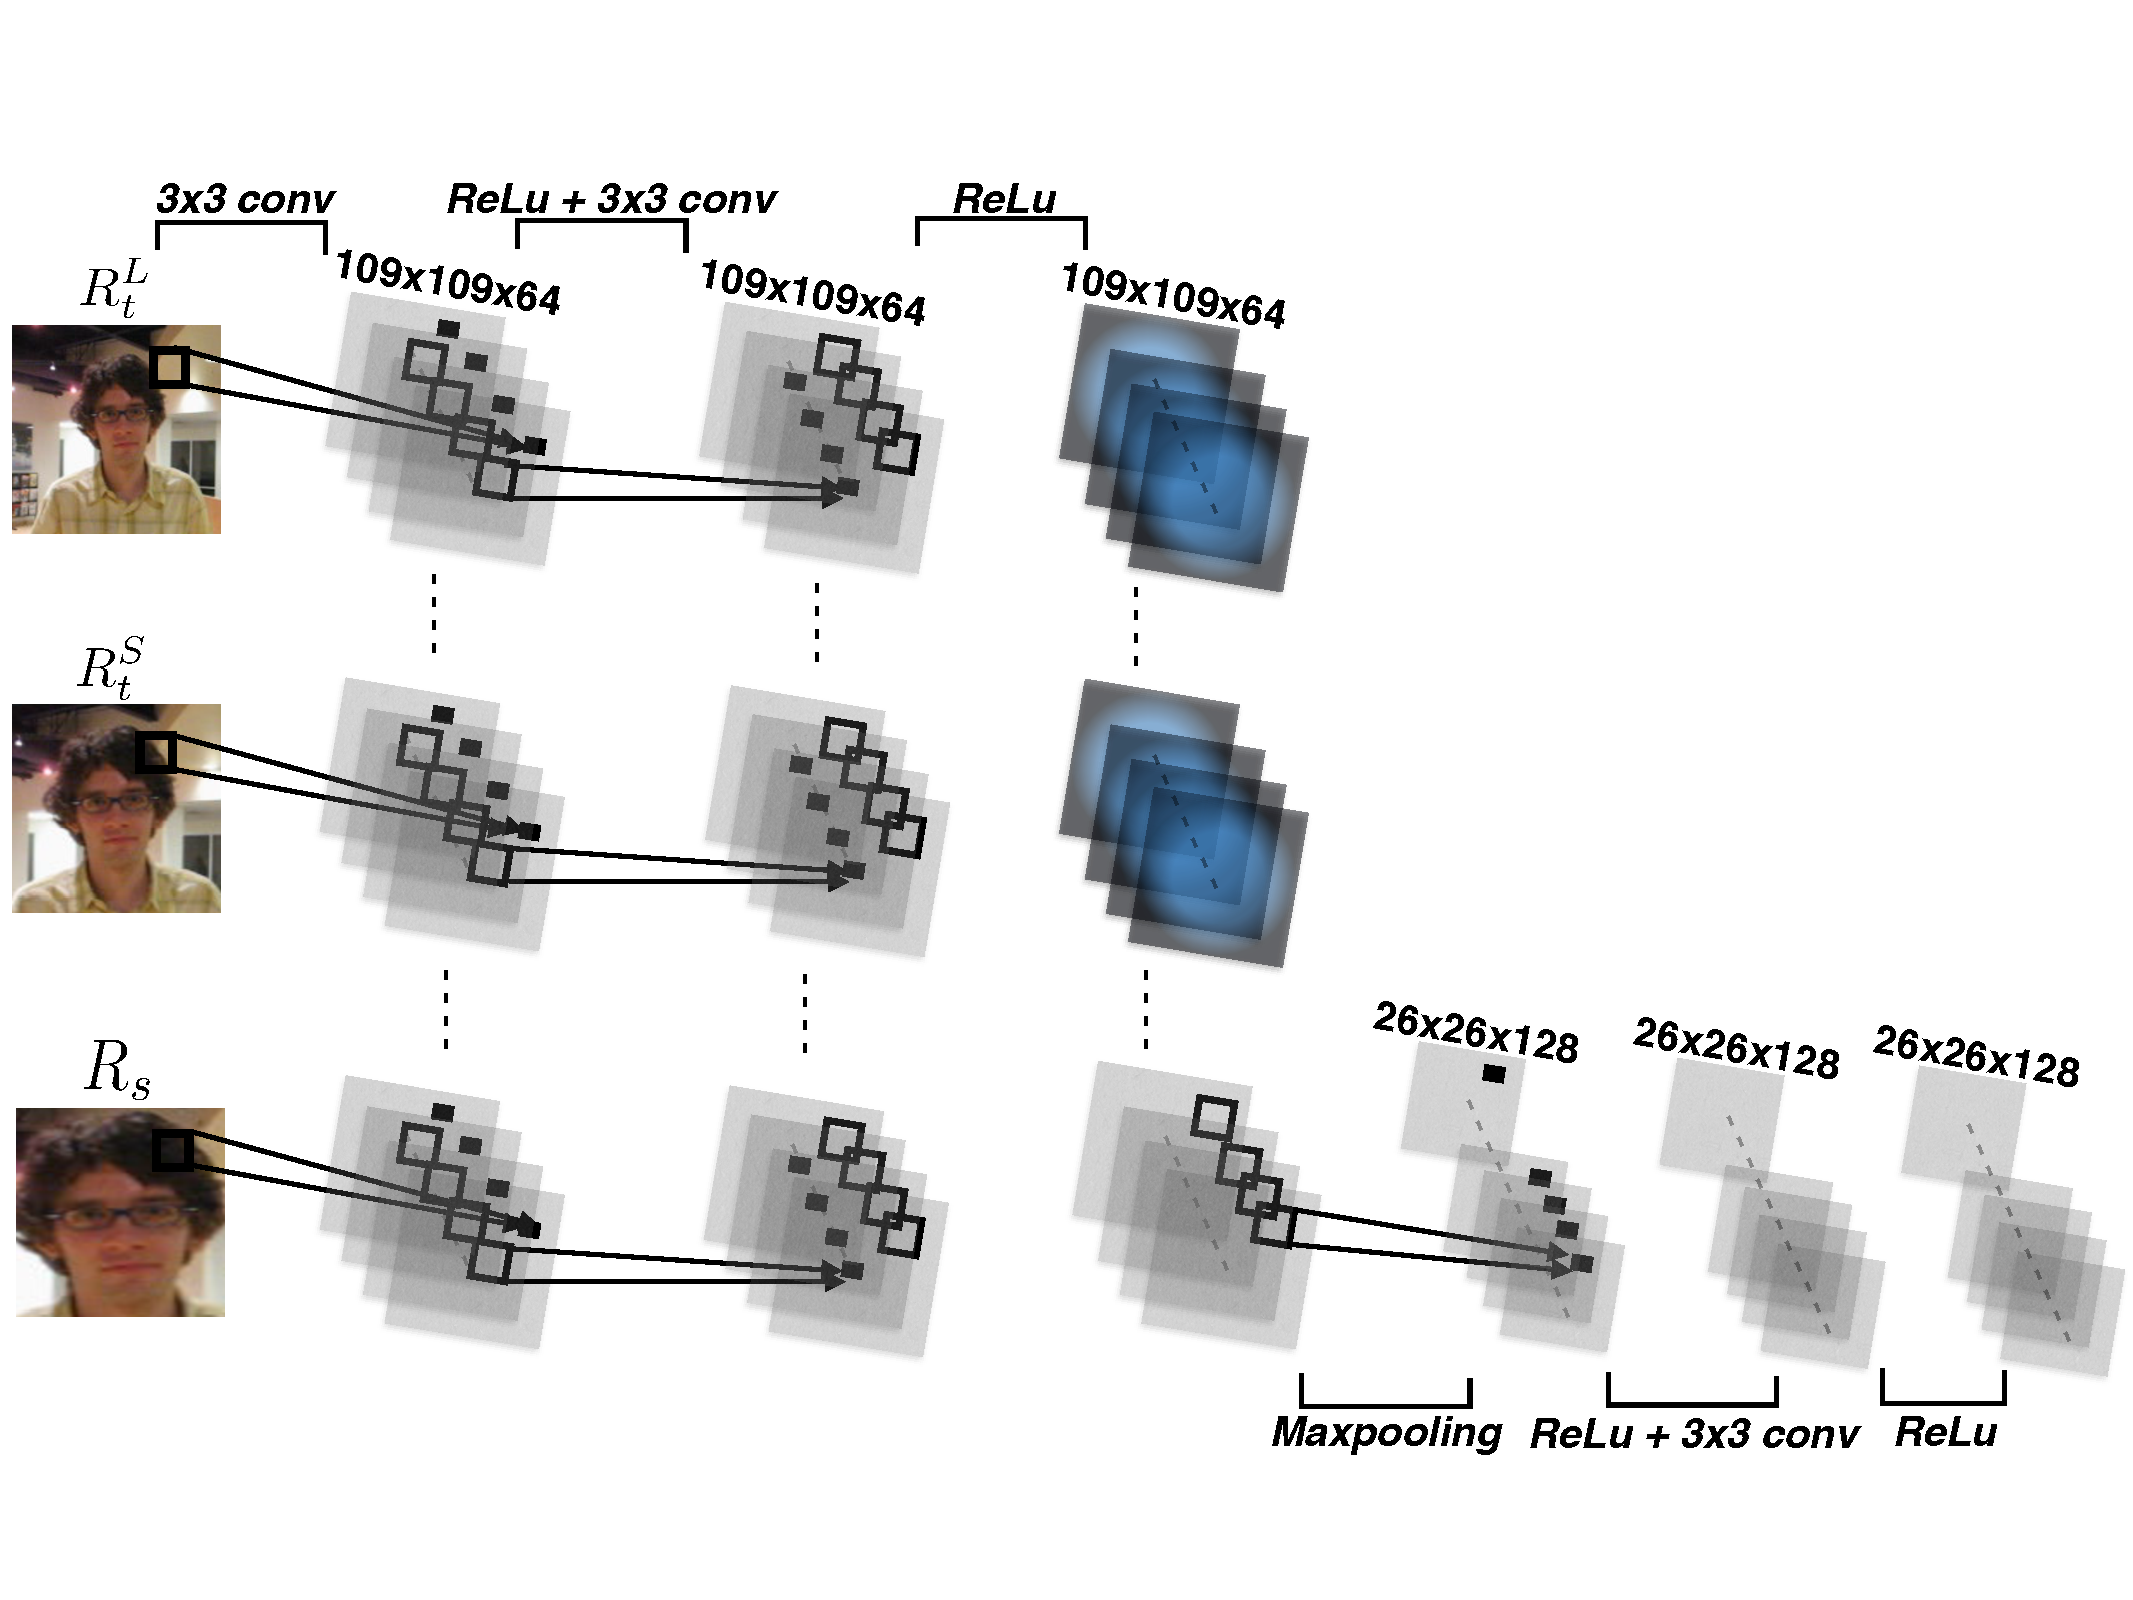
\includegraphics[width=0.48\textwidth]{./figures/Filters_Details_CNN.pdf}
\caption{The proposed conv224-VGGNet feature extraction in Deep{\it
    E}nKCF. $R_{t}^{L}$ and $R_{t}^{s}$ used an hanning window to
  avoid distortion caused by FFT operation whereas $R_{s}$ does not,
  in order to avoid target boundary information loss.}
\label{fig:Filters_CNN}
\end{figure}

\textbf{Particle Filter for Smoothing Transition among KCFs} As
explained earlier, the {\it E}nKCF updates the target's scale at every
other $k$ frames. Although the strategy of updating every other $k$th
frames will result in an optimal run-time performance, this may lead
drifts at the later frames. To prevent such potential drifts, we
developed a Bayes filter that incorporates a target's motion to smooth
any intermediate outputs from individual KCFs. In particular, we use a
particle filter to estimate the target's image coordinate based on the
{\it E}nKCF's outputs. The state in this paper, $\boldsymbol{X_{t}}$,
represents the target's pixel coordinates and its velocity,
$\boldsymbol{X_{t}} = \lbrace x, y, v_{x}, v_{y} \rbrace$, where $x$
and $y$ are the pixel coordinates of the target's centroid, $v_x$ and
$v_y$ are the velocities estimated along the $x$-axis and
$y$-axis. The particle filter predicts, using a motion model with
constant acceleration assumption, the target's next state by
generating a predefined number of particles. Then it uses the
confidence maps of {\it E}nKCF as observation to update its state. The
particle weight is computed as, $w_{p_{t}}(x_{t},y_{t}) =
\sum_{i=1}^{N}\sum_{j=1}^{M} \boldsymbol{y_{R}}(x_{t}-i,y_{t}-j)$,
where $w_{p}$ is the weight of the particle $p$ at time $t$,
$\boldsymbol{y_{R}}$ is the response map from one of the KCFs, and $N$
and $M$ denote the number of rows and columns of the confidence map.
        
%----------------------------------------------------------------------
\section{Experiments} \label{sc:Experiments}
%----------------------------------------------------------------------
So far we explained how the proposed algorithm could efficiently
perform a single-target tracking task while effectively addressing
variations in scale and translation of moving objects. To accurately
evaluate the performance of the proposed algorithm from the
perspective of this paper's goal, we need data with challenging
variations in scale and translation. To this end, we chose the UAV123
data\footnote{\url{https://ivul.kaust.edu.sa/Pages/Dataset-UAV123.aspx}}\cite{mueller2016uav123}
that contains 123 video sequences of objects captured from
low-altitude UAVs. Because of the nature of the video acquisition --
the targets and the camera are moving together, this data pose a great
deal of challenges as the scale and position of the targets change
drastically in most of the sequences. To verify that our algorithm is
useful not only for the image data with such extreme challenges but
also for the one with nominal difficulties in single-object tracking,
we also used the OTB100
data\footnote{\url{http://cvlab.hanyang.ac.kr/tracker_benchmark/benchmark_v10.html}}
\cite{WuLimYang13} that contains the videos recorded from smart phones
and typical cameras in perspective view. In addition, we use the
temporarily down-sampled UAV123 dataset to check how robust our
algorithm is to drastic motions of camera and moving targets. Lastly,
we evaluate the proposed algorithm with deep convolutional features on
the UAV123 dataset to investigate how much performance gain we can
achieve in using deep features over the conventional features like
fHoG and color-naming.

\textbf{Finding Optimal Hyper-parameters} As each of three KCFs in
       {\it E}nKCF is designed to address specific challenges in
       single target tracking problem, the optimal parameters for
       individual KCFs should be different. We set the learning rates
       ($\beta$) of individual filters, $R_{t}^{L}$, $R_{t}^{S}$, and
       $R_{s}$ as $0.020$, $0.020$ and $0.010$. For the kernel of the
       Gaussian neighboring function, we empirically found the optimal
       values of $\alpha$ as $0.7$, $0.6$, and $0.9$ for $R_{t}^{L}$,
       $R_{t}^{S}$, and $R_{s}$. We set the scale filter update
       threshold, $T_{R_{s}}$, to 4, peak-to-sidelobe (PSR) ratio. The
       padding size for the correlation filters is tuned to $2$ for
       $R_{t}^{L}$, $1.50$ for $R_{t}^{S}$, and $0$ for $R_{s}$. For
       our particle filter implementation, we empirically found 1,000
       for the number of particles as an optimal one for balancing the
       run-time performance and accuracy. To keep the level of
       variance among the particles reasonable, we performed the
       re-sampling only when the efficient number of samples,
       $ \hat{N}_{eff} \approx
       (\sum_{p=1}^{P}\boldsymbol{w}_{p}^{2})^{-1} $, is lower than a
       pre-defined threshold.

\begin{figure*}[h]
\centering
\begin{tabular}{ccc}
\tiny\textbf{UAV123}\hspace{.43\linewidth}\textbf{OTB100}\\
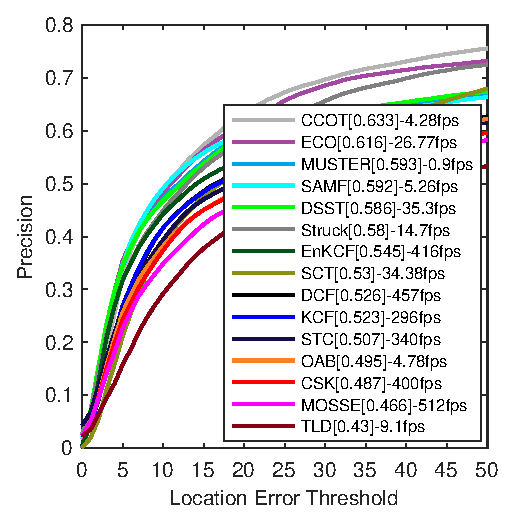
\includegraphics[width=3.80cm]{./figures/pr_uav123.eps}
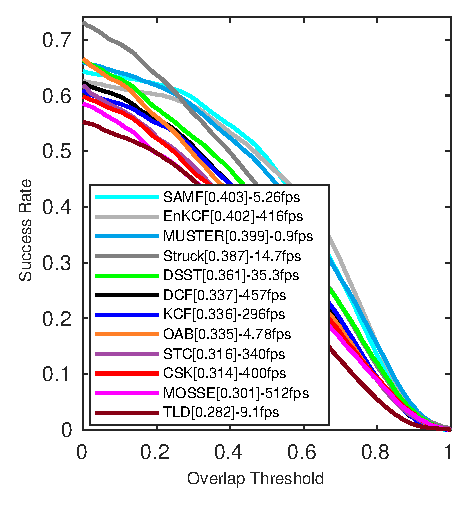
\includegraphics[width=4.10cm]{./figures/sr_uav123.eps}
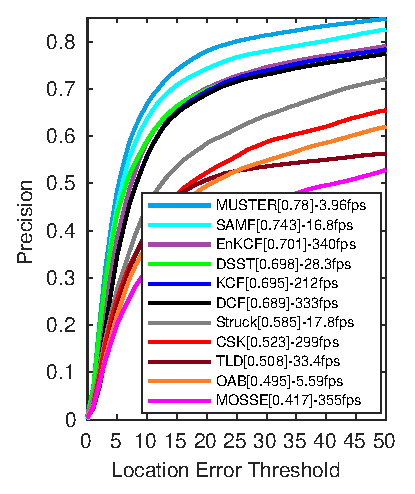
\includegraphics[width=3.80cm]{./figures/pr_otb100.eps}
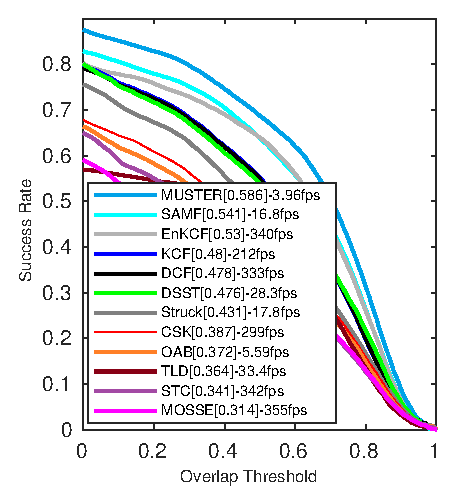
\includegraphics[width=4.10cm]{./figures/sr_otb100.eps}\\
\end{tabular}
\caption{Comparison of {\it E}nKCF's performance with other trackers on the UAV123 and OTB100 datasets.}
\label{fig:UAV123_DATASET}
\end{figure*}

\textbf{Performance on UAV123 Dataset} We used the precision and
success rates to compare the performance of the proposed algorithm
with those of the state-of-the-art tracking algorithms. For the
precision, we rank the trackers based on the precision numbers at 20
pixels whereas in the success rate plots, they are ranked by the area
under curve (AUC) scores. The tracking algorithms under the comparison
include ones at high-speed ($\geq$300 fps): KCF
\cite{henriques2015high}, CSK \cite{henriques2012exploiting}, DCF
\cite{henriques2015high}, MOSSE \cite{bolme2010visual}, and STC
\cite{zhang2014fast} and ones at relatively lower-speed ($\leq$50):
ECO \cite{DanelljanCVPR2017}, CCOT \cite{DanelljanECCV2016}, SCT
\cite{Choi_2016_CVPR}, SAMF \cite{li2014scale}, DSST
\cite{danelljan2014accurate}, Struck \cite{hare2012efficient}, MUSTER
\cite{hong2015multi}, TLD \cite{kalal2012tracking}, and OAB
\cite{zhang2012robust}. The ECO and CCOT trackers originally use deep
convolutional features, however, to perform fair comparison, we use
fHoG and color-naming features similar to our tracker. Figure
\ref{fig:UAV123_DATASET} shows the results on the UAV123 dataset. The
    {\it E}nKCF outperformed other high-speed trackers by $3\%$-$15\%$
    at 20 pixels precision. In particular, three algorithms, SAMF,
    DSST, and Struck did about $5\%$ better than ours in accuracy, but
    10-20 times slower. The more recent trackers, ECO and CCOT, on the
    other hand, outperforms {\it E}nKCF by $15\%$ while running at
    10-15 times slower. For the scale adaptation, {\it E}nKCF did
    fourth best in terms of AUC for the success rate plot. It
    outperformed other high-speed trackers by about $20\%$-$25\%$ in
    AUC. In addition, it performed even better than some of the
    lower-speed trackers.  For example, for AUC, {\it E}nKCF
    outperformed Struck and DSST by $5\%$ and $10\%$ while running at
    more than $10$ and $30$ times faster. For the DSST, we believe our
    algorithm outperformed it because, first of all, the DSST uses a
    1-D scale filter and searches the target's scale over 33
    candidates in a scale pool whereas our algorithm uses a 2-D scale
    filter with 3 candidate scales. Learning a 2-D filter resulted in
    learning more spatial information. Second of all, the DSST uses
    only fHoG whereas our algorithm uses both fHoG and color-naming
    features. Learning complementary features such as color and shape
    provided a better understanding of the ROI.
    
\begin{table*}[!h]
\smaller
\begin{center}
\color{green}--- Best \hspace{.15\linewidth}\color{red}--- $2^{nd}$ Best \hspace{.15\linewidth}\color{blue}--- $3^{th}$ Best \color{black}\\
\resizebox{\textwidth}{!}{\begin{tabular}{|l|c|c|c|c|c|c|c|c|c|}
\hline
Method & {\it E}nKCF & $R_{t}^{S}$+$R_{t}^{L}$+$R_{s}$ & $R_{t}^{L}$+$R_{s}$ & $R_{t}^{S}$+$R_{s}$ & $R_{t}^{L}$* & $R_{t}^{S}$* & $R_{t}^{L}$+$R_{s}$* & $R_{t}^{S}$+$R_{s}$* & $R_{t}^{L}+R_{t}^{S}$+$R_{s}$* \\
\hline\hline
Pr. ($20$px) & \color{blue}53.9 & 48.93 &52.41 & 48.10 & 51.88 & 51.29 & \color{red} 55.85 & 52.14 & \color{green}58.16 \\
SR ($50\%$) & \color{red} 40.2 & 36.75 & 38.23 & 36.04 & 35.12 & 34.43 & \color{blue}39.89 & 38.51 & \color{green}41.58 \\
FPS & \color{red} 416 & \color{blue}412 & 370 & \color{green}425 & 365 & 384 & 135 & 151 & 99 \\
\hline
\end{tabular}}
\end{center}
\caption{Results of running different combinations of the KCFs for
  UAV123 dataset. The '$*$' represents a sequential approach where
  multiple KCFs are, in the given order, applied to every frame like
  in LCT \cite{ma2015long}.}
\label{table:Comparison_to_LCT}
\end{table*}

\textbf{Finding Optimal Combination and Deployment Order of Multiple
  KCFs} In addition to performance comparison with other trackers, we
also conducted an experiment to see what combination and deployment
order of the KCF works best. Table \ref{table:Comparison_to_LCT}
presents results of this experiment. To achieve fair comparison, we
did not use the particle filter. The combination presented at the
$2^{nd}$ column switched the order of deploying $R_{t}^{L}$ and
$R_{t}^{S}$. The one at the $3^{th}$ column removed $R_{t}^{S}$ and
replaces with $R_{t}^{L}$ whereas the one at the $4^{th}$ column
removes $R_{t}^{L}$. The combinations with the ``*'' marker ran the
filters on every frame in the listed order. The trackers at the
$7^{th}$ and $8^{th}$ columns ran a translation and a scale filter on
every frame which is similar to the LCT tracker
\cite{ma2015long}.\footnote{To be precise, the LCT tracker comes with
  a re-detection module for a long-term tracking.} This experiment
empirically verified that the way \textit{E}nKCF uses multiple KCFs is
optimal, in terms of both tracking accuracy and run-time
performance. For example, one could achieve $4.26\%$ higher in
accuracy by running $R_{t}^{L}$ and $R_{t}^{S}$, and $R_{s}$ at every
frame (produced 58.16\% for precision at 20 pixels), but this
combination decreases run-time performance to 317 fps (=416fps -
99fps).

\textbf{Evaluation on Particle Filter Contribution} For the UAV123
dataset, we also evaluated the performance of the {\it E}nKCF with and
without the particle filter. In particular, we use 50 video sequences
with no drastic camera motion. To evaluate the robustness of particle
filter, we add noise from a uniform distribution ($[-20,20]$), to the
translation estimations of the KCFs. For this experiment, the {\it
  E}nKCF with particle filter achieves $51.98\%$ precision at 20
pixels, outperforming the one without particle filter by
$6.32\%$. This experiment validated that the integration of particle
filter into the {\it E}nKCF can further improve the performance.

\textbf{Performance on OTB100 Dataset} Figure \ref{fig:UAV123_DATASET}
shows the results on the OTB100 dataset. The performance of {\it
  E}nKCF on the OTB100 data is similar to that of the UAV123
dataset. Specifically, it performed reasonably well at estimating
target scale in that it showed the highest precision and success rates
among the other high-speed trackers. Interestingly, {\it E}nKCF
outperformed another correlation filter based tracker, DSST, but
performing $5\%$ behind of another low-speed scale adaptive SAMF
tracker. Finally, the ECO, and CCOT achieve $15\%$-$20\%$ higher
precision and success rates than ours while operating at 10-20 times
slower rates.

\textbf{Performance on UAV123$\_$10fps Dataset} We were curious about
how the frame rate of a testing video would affect the performance of
a tracking algorithm. To this end, we use the temporarily down-sampled
version of the UAV123, called UAV123$\_$10fps dataset. The
downsampling of a given video sequence would obviously make the
original UAV123 data more challenging because the displacements of the
moving objects become bigger. To tackle this challenge, we slightly
modified the proposed algorithm -- ran $R_{t}^{L}$ every frame and
removed the particle filter due to larger motion. Figure
\ref{fig:UAV123_10fpsDATASET} shows the performance of the modified
version of {\it E}nKCF and other tracking methods. The precision rates
of the ECO and CCOT dropped about $10\%$ in comparison to the original
UAV123 dataset. Our tracker outperforms other high-speed correlation
filter based trackers including KCF, DSST by about $15\%$-$20\%$ and
showed a precision rate similar to that of SAMF. It ranks as fourth in
AUC while running about $10$ to $100$ times faster than the top three
trackers. It was interesting to observe how sensitive the performance
of the state-of-the-art tracking algorithms is to the frame rate, and,
with a slight modification, the proposed method effectively handled
large displacement of objects in successive frames.

\begin{figure}[!h]
\centering
\begin{tabular}{cc}
\tiny\quad\textbf{UAV123$\_$10fps}\\
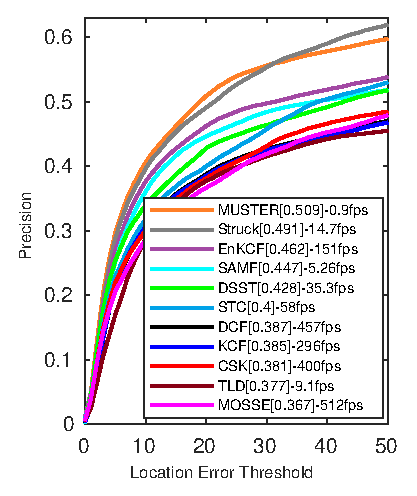
\includegraphics[width=4.02cm]{./figures/pr_uav123_10fps.eps}
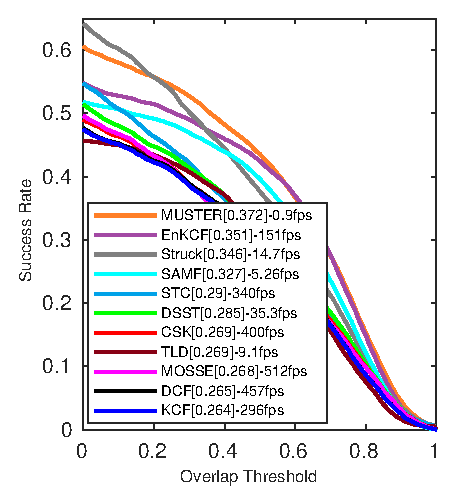
\includegraphics[width=4.00cm]{./figures/sr_uav123_10fps.eps}\\
\end{tabular}
\caption{Comparison of a modified {\it E}nKCF's performance with those
  of the state-of-the-art tracking algorithms on a lower frame rate
  data.}
\label{fig:UAV123_10fpsDATASET}
\end{figure}

\textbf{Evaluation with Deep Features} Our focus so far was to develop
a single-target tracker that does not require offline learning to
effectively address the variations in scale and translation, and can
run at a high-speed, $\ge 300$fps. We would like to see how much the
performance gain we could achieve by replacing the conventional
features, fHoG and color-naming with deep convolutional features. We
use deep convolutional features similar to
\cite{danelljan2015convolutional,ma2015hierarchical}. Note that
running the {\it E}nKCF with deep features would obviously increase
the computational cost and degrade the run-time performance.

Figure \ref{fig:UAV123_DATASET_DeepFeatures} shows the DeepE{\it
  n}KCF's performance on UAV123 dataset. Deep{\it E}nKCF outperformed
the {\it E}nKCF with hand-crafted features by about $3\%$ to $5\%$ in
precision (20 px) and $2\%$ in success rates (AUC). The
\textit{conv224-VGG} setting performed slightly better than the
\textit{conv222-VGG} in precision while achieving similar success rate
(AUC). This indicates that higher level feature abstraction works
better for the smaller ROIs. By using feature abstractions from the
VGGNet pre-trained on millions of images, we can better represent the
low level features of the object than hand-crafted features in
challenging cases such as low contrast ROIs. However, we believe that
the contribution of the deep features is limited by two factors:
increased translational invariance in deeper layers and losing targets
due to large target and camera motion in the UAV123 dataset.

\begin{figure}[!h]
\centering
\begin{tabular}{ccc}
\tiny\quad\quad\textbf{UAV123}\\
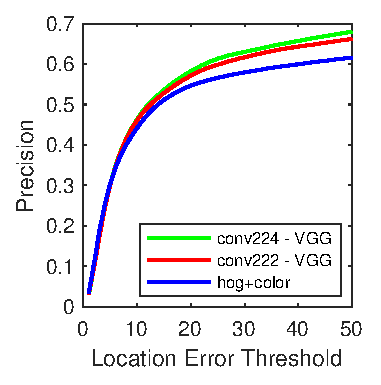
\includegraphics[width=3.60cm]{./figures/pr_deep.eps}
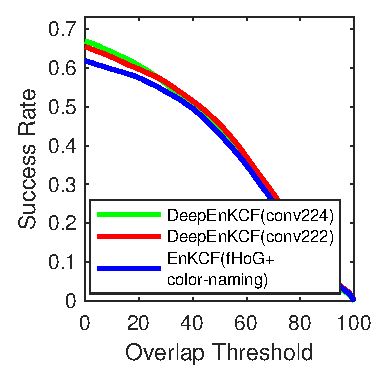
\includegraphics[width=3.70cm]{./figures/sr_deep.eps}\\
\end{tabular}
\caption{Comparison of {\it E}nKCF's ({\it fHoG} + {\it color-naming})
  performance with Deep{\it E}nKCF on the UAV123 dataset. The frame
  rate of the Deep{\it E}nKCF (conv224) was, on average, 30.74 fps and
  the conv222 setting was 35.23 fps on a CPU.}
\label{fig:UAV123_DATASET_DeepFeatures}
\end{figure}

%---------------------------------------------------------------------- 
\section{Conclusion} \label{sc:Conclusion}
%---------------------------------------------------------------------- 
Running a computer vision algorithm on any existing embedded systems
for real-world applications is economically and practically very
attractive. Among other practical considerations, it would be
desirable if such computer vision algorithms require no offline
training and operate at high-speed. To develop a single-target
tracking algorithm to meet these properties, we proposed an extension
of KCF that applies three KCFs, in turn, to address the variations in
scale and translation of moving objects. We also developed a particle
filter to smooth the transition between three KCFs, especially the
transition between the scale and large ROI translation filter. Through
experiments, we found that the way the {\it E}nKCF deployed three KCFs
was optimal, and the particle filter contributed to increase the
performance.  We used two public datasets to evaluate the performance
of the proposed algorithm and other state-of-the-art tracking
algorithms, and found that, on average, the performance of the
proposed algorithm is better than other high-speed trackers over 5\%
on precision at 20 pixels and 10-20\% on AUC. Our implementation ran
at 340 fps for OTB100 and at 416 fps for UAV123 data that is faster
than DCF (333 fps) for OTB100 and KCF (296 fps) for UAV123. Finally,
we explored the idea of utilizing deep features for the proposed
algorithm and found that the deep features helped the proposed
algorithm boost the performance by $5\%$.

Although the proposed algorithm showed a promising result for the
challenging data, we believe the corner case analysis has not been
extensively done yet. As future work, we would like to thoroughly
study under what conditions our algorithm would fail to track
objects. In addition, we also would like to investigate, for long-term
tracking, a way of re-initializing a target when the target is lost,
due to occlusion, illumination change, drastic camera motion, etc.

{\small
\bibliographystyle{ieee}
\bibliography{draft}
}

\end{document}
